\documentclass{article}
\usepackage[utf8]{inputenc}
\usepackage[left=3cm,right=3cm,top=2cm,bottom=2cm]{geometry}
\usepackage[french]{babel}
\usepackage[T1]{fontenc}
\usepackage{lmodern}
\usepackage{graphicx}
\usepackage{amsmath}
\usepackage{minted}
\usepackage{caption}
\usepackage{tikz}
\usepackage{hyperref}

\graphicspath{ {./images/} }
\usetikzlibrary{calc}
\usemintedstyle{borland}
\captionsetup[table]{name=Tableau}

\title{Rapport de TP}
\author{Grégoire DOEBELE }
\date{December 2021}

\begin{document}

\newcommand{\tikzmark}[1]{\tikz[overlay,remember picture] \node (#1) {};}
\newcommand{\DrawBox}[4][]{%
    \tikz[overlay,remember picture]{%
        \coordinate (TopLeft)     at ($(#2)+(-0.2em,0.9em)$);
        \coordinate (BottomRight) at ($(#3)+(0.2em,-0.3em)$);
        %
        \path (TopLeft); \pgfgetlastxy{\XCoord}{\IgnoreCoord};
        \path (BottomRight); \pgfgetlastxy{\IgnoreCoord}{\YCoord};
        \coordinate (LabelPoint) at ($(\XCoord,\YCoord)!0.5!(BottomRight)$);
        %
        \draw [red,#1] (TopLeft) rectangle (BottomRight);
        \node [below, #1, fill=none, fill opacity=1] at (LabelPoint) {#4};
    }
}


\maketitle

\section{Introduction}

L'objectif de ce TP est de se familiariser avec \texttt{scilab} et les interfaces \texttt{C} de \texttt{BLAS} et de \texttt{LAPACK}. 

Tous les codes est disponible sur github :
\newline\noindent
\href{https://github.com/ggdoe/tp-cn-4-ggdoe}{https://github.com/ggdoe/tp-cn-4-ggdoe}\newline
\href{https://github.com/ggdoe/tp-cn-5-ggdoe}{https://github.com/ggdoe/tp-cn-5-ggdoe}

\section{Décomposition LDL\(^t\)}

Rappel,\newline
D'après le cours, on sait que la décomposition \(LDL^t\) existe et est unique pour toute matrice symétrique.

Soit \(A\) symétrique
\[
	A = A^t = 
	\begin{pmatrix}
	a_{1,1}	& \dots	& a_{1,n} 	\\
	\vdots	& \ddots& \vdots	\\
	a_{1,n}	& \dots & a_{n,n} 	\\
	\end{pmatrix}
\]

\(A\) peut s'écrire sous la forme \(LU\) ou \(LDL^t\), avec \(L\) \textit{unit lower triangular}, U \textit{upper triangular} et D diagonale.
En identifiant les termes on trouve que \(U = DL^t\), et les \(L\) sont les même.

\[
	D = 
	\begin{pmatrix}
	&d_1	& 		& 0&	\\
	&		& \ddots& &		\\
	& 0	& 		& d_n & 	\\
	\end{pmatrix}
\]
\[	
	L = 
	\begin{pmatrix}
	1		& 	& 	&  	\\
	l_{2,1}	& \ddots&0& 	\\
	\vdots	& \ddots & \ddots&  \\
	l_{n,1}	& \dots  & l_{n,n-1} & 1 	\\
	\end{pmatrix}, 
	L^t = 
	\begin{pmatrix}
	1		& l_{2,1}& \dots	& l_{n,1} 	\\
			& \ddots&\ddots& \vdots	\\
			& 0 & \ddots& l_{n,n-1} \\
			&  && 1 	\\
	\end{pmatrix}
\]
On obtient donc U simplement en multipliant chaque ligne \(i\) de \(L^t\) par \(d_i\),
\[
	U = DL^t = 
	\begin{pmatrix}
	d_1		& d_1 l_{2,1}& \dots	& d_1 l_{n,1} 	\\
			& \ddots&\ddots& \vdots	\\
			& 0 & \ddots& d_{n-1} l_{n,n-1} \\
			&  && d_n 	\\
	\end{pmatrix}
\]
\[	
	A = LDL^t = 
	\begin{pmatrix}
	1		& 	& 	&  	\\
	l_{2,1}	& \ddots&0& 	\\
	\vdots	& \ddots & \ddots&  \\
	l_{n,1}	& \dots  & l_{n,n-1} & 1 	\\
	\end{pmatrix}\cdot
	\begin{pmatrix}
	d_1		& d_1 l_{2,1}& \dots	& d_1 l_{n,1} 	\\
			& \ddots&\ddots& \vdots	\\
			& 0 & \ddots& d_{n-1} l_{n,n-1} \\
			&  && d_n 	\\
	\end{pmatrix}
\]
Chaque élément \(a_{i,j}\) peut être obtenu en faisant le produit scalaire d'une ligne de L par une colonne de U. Ces matrices étant triangulaire, on peut obtenir le vecteur \texttt{A(j:n,j)} simplement en étendant le vecteur \texttt{L(j,1:j)} en la sous matrice \texttt{L(j:n,1:j)}, comme ci dessous :
\[
	A = 
	\begin{pmatrix}
	a_{1,1}	& \dots 	& a_{1,j} 	& \dots		& a_{1,n} 	\\
	\vdots	& \ddots	& 			&			& \vdots 	\\
	a_{1,j}	& 			& \tikzmark{left}a_{j,j}\ \tikzmark{right0}\  	& 			& a_{j,n}	\\
	\vdots	& 			& \vdots 	& \ddots	& \vdots 	\\
	a_{1,n}	& \dots 	& a_{j,n}\tikzmark{right} 	& \dots 	& a_{n,n} 	\\
	\end{pmatrix}
	\DrawBox[thick, red ]{left}{right}{}
	\DrawBox[very thin, blue ]{left}{right0}{\textcolor{blue}{\Large$\downarrow$}}
	\]
	\[=
	\begin{pmatrix}
	1		& 		 	& 		 	& 			& 		 	\\
	\vdots	& \ddots	& 			&	0		& 	 		\\
	\tikzmark{left}l_{j,1}	& \dots		& 1\quad\tikzmark{right0}		 	& 			& 			\\
	\vdots	& 			& \vdots 	& \ddots	& 	 		\\
	l_{n,1}	& \dots 	& l_{n,j}\tikzmark{right} 	& \dots 	& 1 		\\
	\end{pmatrix}
	\DrawBox[thick, red ]{left}{right}{}
	\DrawBox[very thin, blue ]{left}{right0}{\textcolor{blue}{\Large$\downarrow$}}
	\cdot
	\begin{pmatrix}
	d_{1}	& \dots 	& \tikzmark{left}d_1 l_{j,1} 	& \dots		& d_1 l_{n,1} 	\\
			& \ddots	& \vdots	&			& \vdots 	\\
			& 			& d_{j} \quad\tikzmark{right} 	& 			& d_j l_{n,j}	\\
			& 	0		& 		 	& \ddots	& \vdots 	\\
			& 		 	& 		 	& 		 	& d_{n} 	\\
	\end{pmatrix}
	\DrawBox[thick, red ]{left}{right}{}
\]

On cherche à obtenir $d_j$, en prenant le produit de la j\ieme\ ligne et de la j\ieme\  colonne, on obtient une expression de $a_{j,j}$ :
\texttt{A[j,j] = L[j, 1:j]$\times$(DL$^t$)[1:j,j]}, on note \texttt{v[1:j]} le vecteur \texttt{(DL$^t$)[1:j,j]}.
\[
a_{j,j} = d_j + \sum_{k=1}^{j-1} d_k l^2_{j,k}
\]
Et donc en isolant $d_j$, on obtient l'expression souhaité.
\[
d_j = a_{j,j} - \sum_{k=1}^{j-1} d_k l^2_{j,k}
\]
Pour trouver les valeurs de \(L\), on utilise la même méthode avec les lignes d'en dessous : \texttt{A[j+1:n,j] = L[j+1:n,1:j]$\times$v[1:j]}, on développe puis on isole le vecteur souhaité \texttt{L[j+1:n,j]},
\[
	\begin{array}{r c l}
	\texttt{A[j+1:n,j]} & = & \texttt{d}_j\texttt{L(j+1:n,j) + L[j+1:n,1:j-1]}\times \texttt{v[1:j-1]} \\
	\texttt{d}_j\texttt{L(j+1:n,j)} & = & \texttt{A[j+1:n,j] - L[j+1:n,1:j-1]}\times \texttt{v[1:j-1]}\\
	\texttt{L(j+1:n,j)} & = & \frac{1}{\texttt{d}_j}\texttt{(A[j+1:n,j] - L[j+1:n,1:j-1]}\times \texttt{v[1:j-1])} \\
	\end{array}
\]

Il suffit de calculer pour chaque colonne $d_j$ puis \texttt{L(j+1:n,j)}. Les $d_j$ forment la matrice diagonale D, il ne reste plus qu'a fixé la diagonale de L à 1.

\textcolor{red}{TODO: à finir ??}

Pour tester notre algorithme on a besoin de matrices symétriques, on peut en générer avec \texttt{A = rand(n,n) ; A = A' * A}.
Ainsi \(A\) vérifie bien \(A = A^t\)
\newline\indent

On teste notre algorithme avec la fonction \texttt{myldlt.sci: test\_myldlt()}

\begin{table}[H]
\renewcommand*\arraystretch{1.3}
\begin{center}
\caption{Tests \(LDL^t\)}
\begin{tabular}{|l|c|c|}
  \hline
  n & conditionnement & erreur avant relative \\
  \hline
	4	& \(2.38 \times 10^3\)	& \(2.36 \times 10^{-17}\) \\
	10	& \(9.44 \times 10^5\)	& \(4.27 \times 10^{-17}\) \\
	25	& \(6.93 \times 10^5\)	& \(3.50 \times 10^{-17}\) \\
	50	& \(1.59 \times 10^5\)	& \(2.19 \times 10^{-17}\) \\
	100	& \(2.91 \times 10^7\)	& \(2.39 \times 10^{-17}\) \\
	500	& \(2.44 \times 10^9\)	& \(2.01 \times 10^{-17}\) \\
	1000& \(3.53 \times 10^9\)	& \(1.88 \times 10^{-17}\) \\
  \hline
\end{tabular}
\caption*{\textit{Le conditionnement et l'erreur sont pris avec la 2-norme}}
\end{center}
\end{table}


L'erreur est très faible même pour de grande valeur de \texttt{n} ou un grand conditionnement de \(A\), notre algorithme \(LDL^t\) a une bonne précision.\newline\indent

On souhaite calculer la complexité de notre algorithme \(LDL^t\).\newline
Lors du calcule on écrit directement dans la matrice d'entré, on créé aussi un vecteur de taille n, la complexité en mémoire de notre algorithme est donc de \(n^2+n = \mathcal{O}(n^2)\).\newline
La boucle principale va de \texttt{j = 1:n}, à l'intérieur on a une boucle de \texttt{i = 1:j-1} (qui fait \texttt{2 Read}, \texttt{1 Write}, \texttt{1}\(\times\)), soit un nombre d'opération de l'ordre de \texttt{(j-1)}.\newline
Puis y a un produit scalaire entre deux vecteur de taille \texttt{(j-1)} qui donne aussi un nombre d'opération de l'ordre de \texttt{(j-1)}. \newline
Et enfin il y a un produit entre une matrice \texttt{(n-j)}\(\times\)\texttt{(j-1)} et un vecteur \texttt{(j-1)} soit un nombre d'opération de l'ordre de \texttt{(n-j)(j-1)}.\newline
En sommant entre \texttt{1} et \texttt{n}, on trouve la complexité en temps de l'algorithme,
\[
\sum_{j=1}^n (n-j+2)(j-1) = \mathcal{O}(\frac{n^3}{6}) = \mathcal{O}(n^3)
\]

\textcolor{red}{TODO: préciser la complexité ?}\newline\indent
On teste la complexité en temps notre algorithme avec la fonction \texttt{myldlt.sci: time\_myldlt()}.
\begin{table}[H]
\centering
\footnotesize
\renewcommand*\arraystretch{1.3}
\caption{Complexité en temps \(LDL^t\)}
\begin{tabular}{|l|c|c|r|}
  \hline
  n (nbr répétition) & conditionnement & erreur & temps d'exécution (s)\\
  \hline
	10 (10000)	& \(7.30 \times 10^{7}  \)	& \(3.67 \times 10^{-17} \pm 10^{-18}	\)	& \(6.78 \times 10^{-4} \pm3.05 \times 10^{-4}\) \\
	50 (3000)	& \(2.66 \times 10^{8}  \)	& \(2.58 \times 10^{-17} \pm 10^{-18}	\)	& \(8.86 \times 10^{-3} \pm1.13 \times 10^{-3}\) \\
	100 (1000)	& \(2.97 \times 10^{10} \)& \(2.36 \times 10^{-17} \pm 10^{-18}	\)	& \(3.28 \times 10^{-2} \pm2.82 \times 10^{-3}\) \\
	200 (100)	& \(2.25 \times 10^{9}  \)	& \(2.23 \times 10^{-17} \pm 10^{-18}	\)	& \(1.31 \times 10^{-1} \pm5.30 \times 10^{-3}\) \\
	400 (25)	& \(8.68 \times 10^{9}  \)	& \(2.16 \times 10^{-17} \pm 10^{-19}	\)	& \(6.03 \times 10^{-1} \pm6.13 \times 10^{-2}\) \\
	500 (15)	& \(4.47 \times 10^{9}  \)	& \(1.97 \times 10^{-17} \pm 10^{-19}	\)	& \(9.97 \times 10^{-1} \pm2.62 \times 10^{-2}\) \\
	800 (5)		& \(6.25 \times 10^{10} \)	& \(2.16 \times 10^{-17} \pm 10^{-19}	\)	& \(3.23 \pm3.39 \times 10^{-2}\) \\
	1000 (5)	& \(1.85 \times 10^{10} \)	& \(1.90 \times 10^{-17} \pm 10^{-19}	\)	& \(6.18 \pm8.89 \times 10^{-1}\) \\
  \hline
\end{tabular}
\caption*{\textit{On utilise les fonctions }\texttt{mean}\textit{ et }\texttt{stdev} \textit{pour calculer la moyenne et l'écart-type de l'erreur et du temps d'exécution.}}
\end{table}

On trace la variation du temps d'exécution avec la fonction \texttt{myldlt.sci: plot\_time\_myldlt()}.

\begin{figure}[H]
\caption{Temps d'exécution \(LDL^t\)}
\centering
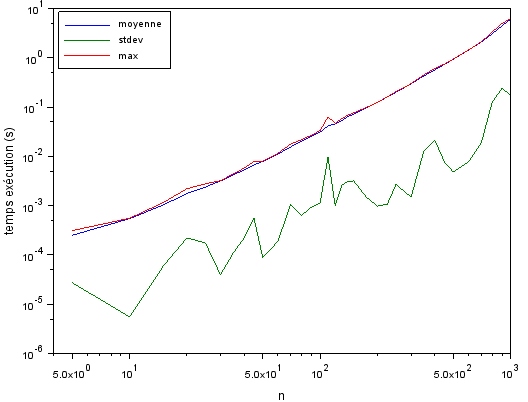
\includegraphics[scale=0.80]{time_LDLt}
\end{figure}
Dans un graphique \(\log\log\), les fonctions \(x^k\) apparaissent comme des droites de pente \(k\). Ici la courbe de la moyenne à une pente d'environ \(2\), ce qui est significativement moins que la valeur théorique \(\mathcal{O}(n^3)\). C'est très certainement dû aux optimisations de \texttt{BLAS/LAPACK}, cependant on remarque que la courbe n'est pas tous à fait linéaire, vers les grandes valeur de \(n\) la pente devient supérieur à \(2\).

On compare \(LDL^t\) et \(LU\) (sans pivot partiel) avec la fonction \texttt{myldlt.sci: comp\_mylu\_myldlt()}

\begin{table}[H]
\centering
\renewcommand*\arraystretch{1.3}
\caption{Comparaison \(LDL^t\ -\ LU\)}
\begin{tabular}{|l|c|c|c|}
  \hline
  n & erreur & temps exécution \(LDL^t\) (s) & temps exécution \(LU\) (s) \\
  \hline
	5	&	\(5.81 \times 10^{-16}\)	&	\(2.69 \times 10^{-4}\)	&	\(1.83 \times 10^{-4}\) \\
	10	&	\(2.18 \times 10^{-15}\)	&	\(6.58 \times 10^{-4}\)	&	\(3.21 \times 10^{-4}\) \\
	25	&	\(1.21 \times 10^{-14}\)	&	\(2.47 \times 10^{-3}\)	&	\(9.59 \times 10^{-4}\) \\
	50	&	\(3.64 \times 10^{-14}\)	&	\(8.24 \times 10^{-3}\)	&	\(2.75 \times 10^{-3}\) \\
	100	&	\(1.39 \times 10^{-13}\)	&	\(3.04 \times 10^{-2}\)	&	\(1.23 \times 10^{-2}\) \\
	200	&	\(5.66 \times 10^{-13}\)	&	\(1.27 \times 10^{-1}\)	&	\(7.22 \times 10^{-2}\) \\
	300	&	\(1.62 \times 10^{-12}\)	&	\(2.99 \times 10^{-1}\)	&	\(2.19 \times 10^{-1}\) \\
	500	&	\(3.98 \times 10^{-12}\)	&	\(9.47 \times 10^{-1}\)	&	\(1.21\) \\
	750	&	\(8.12 \times 10^{-12}\)	&	\(2.69\)				&	\(4.88\) \\
	1000 &	\(1.54 \times 10^{-11}\)	&	\(6.61\) 				&	\(12.8\) \\
  \hline
\end{tabular}
\caption*{\textit{L'erreur est la 2-norme de la différence entre \(LDL^t\) et \(LU\)}}
\end{table}

On remarque que sur de petite matrice \(LU\) est plus rapide, mais que sur de grande matrice c'est \(LDL^t\) qui est plus rapide. L'algorithme \(LU\) a une complexité du même ordre que \(LDL^t\) mais il fait un peu plus de calculs dans la boucle principale :  \begin{minted}{scilab}
// boucle principale LU
A(k+1:n, k+1:n) = A(k+1:n,k+1:n) - A(k+1:n,k) * A(k,k+1:n)
// boucle principale LDLt
A(j+1:n,j) = (A(j+1:n,j) - A(j+1:n,1:j-1) * v(1:j-1))/A(j,j)
\end{minted}
On peut expliquer que notre algorithme \(LU\) est plus rapide sur de petites valeurs de \(n\) par sa compacité. Il n'y a qu'une boucle et on utilise presque exclusivement les opérations vectorielles de \texttt{scilab}, le code est fortement optimisé, mais ça ne suffit pas pour battre \(LDL^t\) sur de grandes matrices.

\section{CSR}

Pour implémenter un algorithme de multiplication d'une matrice creuse au format CSR, on regarde comment se présente une matrice CSR.

Soit \(A\) une matrice creuse, tel que :
\[
A = 
\begin{pmatrix}
	0	&	0	&	0	&	0	& 0	\\
	0	&	9	&	13	&	0	& 0	\\
	0	&	0	&	0	&	11	& 0	\\
	12	&	0	&	0	&	0	& 0	\\
	0	&	0	&	0	&	0	& 9	\\
	0	&	3	&	0	&	0	& 0	\\
	5	&	0	&	0	&	0	& 0	\\
\end{pmatrix}
\]

Au format CSR, elle se présente sous cette forme :
\[
\texttt{AA}  = 
\begin{bmatrix}
9	&	13	&	11	&	12	&	9	&	3	&	5	\\
\end{bmatrix}
\]
\[
\texttt{JA}  = 
\begin{bmatrix}
2	&	3	&	4	&	1	&	5	&	2	&	1	\\
\end{bmatrix}
\]
\[
\texttt{IA}  = 
\begin{bmatrix}
1	&	1	&	3	&	4	&	5	&	6	&	7	&	8	\\
\end{bmatrix}
\]

\texttt{AA} contient les valeurs, \texttt{JA} le numéro de la colonne de la valeur associer, et \texttt{IA} l'index des sauts de lignes (index des éléments \texttt{AA} et \texttt{JA}). \texttt{IA} commence toujours par 1, lorsqu'une ligne est sauté (ligne de 0) l'index est répété dans \texttt{IA}, par exemple ici : la première ligne est sauté, donc après le premier \(1\) obligatoire, on met un second \(1\).

On remarque qu'au format CSR, la taille du vecteur \texttt{IA} est la même que celle du \texttt{nombre de lignes + 1}, le vecteur de sorti du produit \(Ax\) aura donc un nombre d'élément égal à \texttt{length(IA)-1}

Soit \(x\) un vecteur, on souhaite faire le produit matrice-vecteur \(Ax\), le vecteur x soit avoir le même nombre d'élément que le nombre de colonne de \(A\).
La boucle principale de l'algorithme de multiplication CSR doit se faire sûr le nombre d'élément non nul de A, à l'intérieur de celle ci on place une boucle while qui incrémentera l'indicateur de la ligne actuelle tant que \texttt{IA} nous dit de sauter de ligne. Le produit scalaire se fait élément par élément, l'élément \texttt{AA(i)} est positionner à la colonne \texttt{JA(i)} donc on sait par quel élément de \(x\) on doit le multiplier \texttt{x(JA(i))}. La complexité de l'algorithme est en \(\mathcal{O}(\texttt{nombre\ éléments\ non\ nul})\).

\begin{scriptsize}
\centering
\begin{minted}{scilab}
function [v] = csr_mv(AA, JA, IA, x)
    n = length(JA)
    v = zeros(length(IA)-1,1)
    k = 1 // ligne actuelle
    for i=1:n
        while(i == IA(k+1)) // saute les lignes nulles
            k = k + 1
        end
        v(k) = v(k) + AA(i) * x(JA(i))
    end
    if(isrow(x)) // col/row coherente avec x
        v = v'
    end
endfunction
\end{minted}
\end{scriptsize}

Pour tester cet algorithme, on a besoin de pouvoir générer des matrices creuses, et calculer leur forme CSR.

Un moyen efficace pour généré des matrices creuse est de remplir une matrice vide de quelques valeurs aléatoires, puis de permuter aléatoirement ses éléments. Pour cela on utilise la fonction \texttt{grand(1, "prm", A)} de \texttt{scilab}, le \texttt{"prm"} signifie qu'on souhaite une permutation, le 1 signifie que l'on en veut qu'une seule, et \texttt{A} est la matrice à permuter. Voir l'implémentation dans \texttt{csr.sci: make\_mat\_creuse}.
\newline\indent

L'algorithme pour calculer le format CSR est aussi très simple. On parcours \(A\) avec deux boucle fort (selon les lignes), on note les valeurs non nulle dans \texttt{AA}, les colonnes dans \texttt{JA}, et lorsqu'on change de ligne on mets d'indice dans \texttt{IA}. Cependant étant donné qu'on doit parcourir toutes les cases de \(A\), cet algorithme est en \(\mathcal{O}(n^2)\). Voir l'implémentation dans \texttt{csr.sci: make\_csr(A)}.

On peut tester cet algorithme en faisant et défaisant la forme CSR (avec la fonction \texttt{csr.sci: undo\_csr(..)}), puis en prenant la 2-norme de la matrice initiale moins celle qui a été fait puis défait. On trouve que ces matrices sont toujours identique quelque soit la taille de la matrices initiale. Voir l'implémentation dans \texttt{csr.sci: test\_csr()}
\newline\indent

On peut maintenant tester la multiplication matrice creuse vecteur. On génère d'abord une matrice creuse \texttt{n}\(\times\)\texttt{m} avec la fonction \texttt{make\_mat\_creuse}, on génère aussi un vecteur creux \texttt{m}\(\times\)\texttt{1} avec la même fonction. On converti cette matrice en CSR avec \texttt{make\_csr}, puis on récupère le vecteur sortie de \texttt{csr\_mv} que l'on compare avec \(Ax\) (en prenant la 2-norme de la différence). Voir l'implémentation dans \texttt{csr.sci: test\_csr\_mv()}

Même pour des matrices très grande (\(5000\times3000\)), la différence entre les solutions est toujours nulle. L'algorithme \texttt{csr\_mv} donne donc un résultat correct.

On peut comparer les performances de \texttt{csr\_mv} avec \texttt{Ax}. Pour de grandes matrices, la majorité du temps est perdu en calculant le format CSR avec la fonction \texttt{make\_csr} (qui est en \(\mathcal{O}(n^2)\)). 

\begin{table}[H]
\caption{Comparaison \texttt{csr\_mv - Ax}}
\renewcommand*\arraystretch{1.3}
\begin{tabular}{|l|c|c|c|}
  \hline
  n\(\times\)m & temps exécution \texttt{csr\_mv} (s) & temps exécution \(Ax\) (s) \\
  \hline
	\(5 \times 5\)		&	\(6.62 \times 10^{-5}\)	&	\(3.80 \times 10^{-6}\)	\\
	\(25 \times 25\)	&	\(4.63 \times 10^{-4}\)	&	\(4.60 \times 10^{-6}\)	\\
	\(75 \times 40\)	&	\(1.79 \times 10^{-3}\)	&	\(6.10 \times 10^{-6}\)	\\
	\(100 \times 100\)	&	\(5.64 \times 10^{-3}\)	&	\(1.06 \times 10^{-5}\)	\\
	\(500 \times 325\)	&	\(9.88 \times 10^{-2}\)	&	\(1.37 \times 10^{-4}\)	\\
	\(2500 \times 1200\)&	6.08					&	\(2.14 \times 10^{-3}\)	\\
	\(5000 \times 3000\)&	29.0					&	\(1.07 \times 10^{-2}\)	\\
  \hline
\end{tabular}
\caption*{\textit{On vérifie systématiquement que les deux vecteurs résultats sont identiques.}}
\end{table}



On remarque que le produit matrice-vecteur natif de \texttt{scilab} est dans tous les cas plus performant, que notre \texttt{csr\_mv}. Notre fonction est interprété par \texttt{scilab} c'est ce qui fait qu'elle est moins performante. Dans un langage compilé comme C, le produit matrice-vecteur CSR serait plus rapide que le produit matrice-vecteur classique.

\section{Poisson 1D}

L'équation de la chaleur 1D s'écrit :
\[
	\left \{
	\begin{array}{r c l}
		-k \frac{\partial^2 T}{\partial x^2} & = & g,\quad x \in ]0,1[ \\
		T(0) & = & T_0 \\
		T(1) & = & T_1 \\
	\end{array}
	\right .
\]
En faisant un développement Taylor, on obtient :
\[
	\left \{
	\begin{array}{r c l}
		T(x+h) & = & T(x) + hT'(x) + \frac{h^2}{2} T''(x) + o(h^3)\\
		T(x-h) & = & T(x) - hT'(x) + \frac{h^2}{2} T''(x) + o(h^3)\\
	\end{array}
	\right .
\]
On additionne ces deux equations pour supprime le terme $T'$, puis on isole $T''$.
\[
	\begin{array}{r c l}
		T(x-h)+T(x+h) & = & 2T(x) + h^2 T''(x) + o(h^3)\\
	\end{array}
\]
\[
	\begin{array}{r c l}
		T''(x) & = & \frac{T(x-h) - 2T(x) + T(x+h)}{h^2}  + o(h)\\
	\end{array}
\]
On discrétise l'espace en $n+2$ points avec $h$ le pas.
\[
	\begin{array}{r c l}
	h & = & \frac{x_{max} - x_{min}}{n-1} = \frac{1}{n+1} \\
	x_i & = & ih \\
	T(x_i) & = & T_i \\
	\end{array}
\]
On peut donc écrire :
\[
	\begin{array}{r c c c l}
	T(x_i + h) & = & T(x_{i+1}) & = & T_{i+1} \\
	T(x_i - h) & = & T(x_{i-1}) & = & T_{i-1} \\
	\end{array}
\]
\[
	\begin{array}{r c l}
		T''(x_i) & = & \frac{T_{i-1} - 2T_i + T_{i+1}}{h^2}  + o(h)\\
	\end{array}
\]
\[
	\begin{array}{r c c c l}
		-T_{i-1} + 2T_i - T_{i+1} & = & \frac{h^2g(x_i)}{k} & = & \frac{g_i}{k(n+1)^2}\\
	\end{array}
\]
On obtient donc un système d'équation linéaire qu'on peut représenter par une matrice.
\[
	u = 
	\begin{bmatrix}
		T_1 & T_2 & \cdots & T_{n-1} & T_n \\
	\end{bmatrix}^t
\]
\[
	A = 
	\begin{pmatrix}
	2	& 	-1	&	0	& 0	\\
	-1	&	2	&\ddots	& 0	\\
	0	& \ddots&\ddots	&-1	\\
	0	& 	0	& -1 	& 2	\\
	\end{pmatrix}
	\quad u = 
	\begin{pmatrix}
		T_1 \\ T_2 \\ \cdots \\ T_{n-1} \\ T_n \\
	\end{pmatrix}
\]
\[
	f = \frac{1}{k(n+1)^2}
	\begin{pmatrix}
		g_1 \\ g_2 \\ \vdots \\ g_{n-1} \\ g_n \\
	\end{pmatrix}
\]
Cependant y a des problèmes aux bord, on est censé avoir :
\[
	\begin{array}{r c l}
		-T_0 + 2T_1 - T_2 & = & \frac{g_1}{k(n+1)^2}\\
		-T_{n-1} + 2T_n - T_1 & = & \frac{g_n}{k(n+1)^2}\\
	\end{array}
\]
On doit donc ajouter un terme correctif à $f$ :
\[
	\begin{bmatrix}
		T_0 & 0 & \cdots & 0 & T_1 \\
	\end{bmatrix}^t
\]
\[
	f = \frac{1}{k(n+1)^2}
	\begin{pmatrix}
		g_1 \\ g_2 \\ \vdots \\ g_{n-1} \\ g_n \\
	\end{pmatrix} 
	+ \begin{pmatrix}
		T_0 \\ 0 \\ \vdots \\ 0 \\ T_1 \\
	\end{pmatrix}
\]
En posant $g=0$ on obtient :
\[
	g = 0 \quad	\Longrightarrow \quad 
	f = \begin{pmatrix}
		T_0 \\ 0 \\ \vdots \\ 0 \\ T_1 \\
	\end{pmatrix}
\]
De plus l'équation différentielle se simplifie en :
\[
	\frac{\partial^2 T}{\partial x^2} = 0
\]
Ça implique que $T$ est linéaire en $x$, les conditions aux limites imposent que 
\[
	T(x) = T_0 + x(T_1 - T_0)
\]

Pour trouver notre inconnue $u$, il suffit de résoudre le système \(Au = f\). On a avantage à profiter du fait que $A$ soit une matrice tridiagonale. On pourra mesurer efficacement l'erreur grâce à la solution analytique.

\section{Résolution Poisson 1D méthode directe}

\texttt{BLAS} et \texttt{LAPACK} sont des bibliothèques \texttt{FORTRAN}, leurs interfaces \texttt{C} sont nommées respectivement \texttt{CBLAS} et \texttt{LAPACKE}. Leur \textit{header} sont inclus dans notre \texttt{blaslapack\_headers.h}. \texttt{lib\_poisson1D.c} contient les fonctions qui nous permettrons d'initialiser nos matrices (poisson 1D et identité) et nos vecteurs (discrétisation de l'espace 1D, vecteur \texttt{f}, et solution analytique). Le fichier contient également les fonctions qui permettent d'écrire dans un fichier les différents vecteur et matrices, ainsi que des fonctions qui seront utile pour résoudre le problème par méthode itérative.

Le fichier \texttt{tp\_env.c} permet de vérifier que \texttt{BLAS/LAPACK} est correctement installé sur la machine. Elle affiche différentes constantes de \texttt{float.h}, puis effectue une copie d'un tableau de double à l'aide de la fonction \texttt{cblas\_dcopy}.

\begin{scriptsize}
\begin{minted}{c}
void cblas_dcopy(const int N, const double *X, const int incX, double *Y, const int incY);
\end{minted}
\end{scriptsize}
\texttt{N} est le nombre d'élement du tableau X à copier dans Y, \texttt{incX} (resp. \texttt{incY}) est l'incrément qu'on doit ajouter à l'index pour chaque élément (en partant de 0). Par exemple, si on veut copier les éléments \texttt{X[0]}, \texttt{X[3]}, $\cdots$, \texttt{X[3N]} alors \texttt{incX} est égale à $3$.

La résolution par méthode directe utilise la fonction \texttt{dgbsv} de \texttt{LAPACK}, cette fonction résout un système de la forme $Ax = b$ d'inconnue $x$ par factorisation LU (avec \texttt{dgbtrf}) \footnote{dgbsv : \href{http://www.netlib.org/lapack/explore-html/d3/d49/group__double_g_bsolve_gafa35ce1d7865b80563bbed6317050ad7.html}{http://www.netlib.org/lapack/explore-html/[...]0ad7.html}} puis le résout avec \texttt{dgbsv}.

Avant d'appeler cette fonction plusieurs étape sont nécessaires. On déclare nos vecteurs (\texttt{X}, \texttt{RHS}, \texttt{EX\_SOL}) et on alloue la place à l'aide de \texttt{malloc}, nos trois vecteur comportent \texttt{*la} éléments. On discrétise notre espace \texttt{X} (sur \texttt{*la + 2} points) avec la fonction :
\begin{scriptsize}
\begin{minted}{c}
void set_grid_points_1D(double* x, int* la);
\end{minted}
\end{scriptsize}
Puis on initialise le vecteur \texttt{f} ($Au = f$) ici appelé RHS, avec la fonction : \begin{scriptsize}
\begin{minted}{c}
void set_dense_RHS_DBC_1D(double* RHS, int* la, double* BC0, double* BC1);
\end{minted}
\end{scriptsize}
qui remplit de zéro les \texttt{*la} éléments de \texttt{RHS} excepter pour le premier et le dernier élément où elle mets respectivement \texttt{*BC0} et \texttt{*BC1}.

Il ne reste plus qu'à initialiser la matrice $A$, pour appeler \texttt{d\textcolor{red}{gb}sv}, la matrice doit être stocker sous format \textit{band}.
En stockage \textit{band}, on ne stocke que les diagonales de la matrice. On écrit sous forme de matrice les diagonales de A. On aligne à droite les diagonales supérieurs en laissant vide les premiers éléments (et alignement à gauche pour les diagonales inférieurs).
\[
\begin{pmatrix}
		2	& 	-1	&	0	& 0	\\
		-1	&	2	&\ddots	& 0	\\
		0	& \ddots&\ddots	&-1	\\
		0	& 	0	& -1 	& 2	\\
	\end{pmatrix}
	\Longrightarrow
	\begin{pmatrix}
		\ast& 	-1	&	-1	&	\cdots	&	-1	&	-1	\\
		2	& 	2	&	2	&	\cdots	&	2	&	2	\\
		-1	& 	-1	&	-1	&	\cdots	&	-1	&	\ast\\
	\end{pmatrix}
\]
D'après la documentation de \texttt{LAPACK}\footnote{Stockage Band LAPACK : \href{https://www.netlib.org/lapack/lug/node124.html}{https://www.netlib.org/lapack/lug/node124.html}}, les éléments $\ast$ n'ont pas besoin d'être initialiser à 0.
La même page de documentation nous informe que lorsque qu'on effectue une factorisation \texttt{LU}, on a besoin d'allouer \texttt{*kl} diagonales supérieurs additionnelle. Pour poisson 1D, notre matrice possède 1 diagonale inférieur (\texttt{*kl}) et 1 supérieur (\texttt{*ku}). Pour la factorisation \texttt{LU}, il faut donc au total réserver 1 diagonale inférieur, 1 diagonale principale, et 2 diagonales supérieurs.
\[ 
	\Longrightarrow
	\begin{pmatrix}
		\ast& \ast	&	\texttt{+}	&	\cdots	&	\texttt{+}	&	\texttt{+}	\\
		\ast& 	-1	&	-1	&	\cdots	&	-1	&	-1	\\
		2	& 	2	&	2	&	\cdots	&	2	&	2	\\
		-1	& 	-1	&	-1	&	\cdots	&	-1	&	\ast\\
	\end{pmatrix}
\]
D'après la documentation de la \texttt{MKL}\footnote{MKL Matrix Arguments : \href{https://www.smcm.iqfr.csic.es/docs/intel/mkl/mkl_manual/appendices/mkl_appB_MA.htm}{https://www.smcm.iqfr.csic.es/docs/intel/mkl/[...]\_MA.htm}} les éléments \texttt{+} n'ont pas besoin d'être initialiser, et les éléments $\ast$ ne sont pas utiliser par \texttt{dgbsv}. On pourrait donc théoriquement stocker ce qu'on veut à la place des $\ast$, et ces valeurs ne seront pas affectées par \texttt{dgbsv}.

Cette matrice sera ensuite stockée dans un tableau 1D, il y a deux méthodes, soit on stocke les éléments en lisant la matrice ligne par ligne (\texttt{Row Major}), soit colonne par colonne (\texttt{Col Major}) (de gauche à droite et de haut en bas).
\[ 
	exemple : \texttt{Col Major} \Longrightarrow
	\begin{bmatrix}
	\ast & \ast	& 2 & -1 & \cdots & \texttt{+} & -1 & 2 & \ast
	\end{bmatrix}
\]
On appelle ce tableau \texttt{AB} (\texttt{A band}), on doit alloué \texttt{la(2kl+ku+1)} éléments.
On peut maintenant appeler \texttt{dgbsv}.
\begin{scriptsize}
\begin{minted}{c}
int LAPACKE_dgbsv( int matrix_layout, int n, int kl, int ku, int nrhs, 
                   double* ab, int ldab, int* ipiv, double* b, int ldb );
\end{minted}
\end{scriptsize}
\begin{itemize}
\item On doit indiquer le mode de stockage de notre matrice \textit{band} (\texttt{matrix\_layout}) : soit \\ \texttt{LAPACK\_ROW\_MAJOR}, soit \texttt{LAPACK\_COL\_MAJOR}.
\item \texttt{n}, \texttt{kl} et \texttt{ku} sont la taille de notre matrice et le nombre de diagonale.
\item \texttt{nrhs} est le nombre de vecteur avec lesquels on veut résoudre le système (avec des \texttt{RHS} différents), ici on n'a qu'un seul \texttt{RHS}.
\item \texttt{ab} est notre matrice au format \texttt{matrix\_layout}.
\item \texttt{ldab} est la \texttt{leading dimension} de \texttt{ab}, c'est-à-dire le nombre d'élément  séparant deux lignes consécutive en mémoire pour la même colonne. En \texttt{Row Major} il y a \texttt{la} éléments séparant deux lignes, et en \texttt{Col Major} il y en a $\texttt{2kl+ku+1 = lab}$.
\item \texttt{ipiv} stocke les index des pivots de la factorisation \texttt{LU}, on doit donc alloué préalablement \texttt{ipiv} avec \texttt{la} éléments. Dans le code on alloue avec \texttt{calloc} qui initialise chaque éléments avec 0.
\item \texttt{b} est notre \texttt{RHS}, et \texttt{ldb} est la \texttt{leading dimension} de b, donc 1 en \texttt{Row Major} et \texttt{la} en \texttt{Col Major}.
\end{itemize}
La fonction écrit la solution directement dans \texttt{RHS}.
Elle retourne 0 pour un succès, sinon elle renvoie un nombre \texttt{<0} en cas d'erreur dans un des arguments d'appel de la fonction, ou \texttt{>0} si la solution n'a pas pu être calculer. On stocke cette valeurs dans \texttt{info} qu'on affiche après l'appel de la fonction.

Pour vérifier la solution, on la compare avec la solution analytique. On doit d'abord remettre en ordre la permutation de la factorisation \texttt{LU}, par chance \texttt{ipiv} représente la permutation identité, on peut donc comparer directement \texttt{RHS} et \texttt{EX\_SOL}. On calcule l'erreur commise :
\[
	\frac{\lVert ex\_sol - rhs \rVert_2}{\lVert rhs \rVert_2}
\]
On doit donc faire 2 produits scalaires, et 1 \texttt{daxpy}. On utilise les fonctions de \texttt{BLAS 1} :
\begin{scriptsize}
\begin{minted}{c}
double cblas_ddot(const int N, const double *X, const int incX, const double *Y, const int incY);
void cblas_daxpy(const int N, const double alpha, const double *X, const int incX, 
						double *Y, const int incY);
\end{minted}
\end{scriptsize}
Ces fonctions s'utilisent de la même manière que \texttt{cblas\_dcopy} plus haut (\texttt{incX} et \texttt{incY}). Le résultat de \texttt{cblas\_ddot} est renvoyé par valeur retour, \texttt{cblas\_daxpy} stocke le résultat dans \texttt{y}.
\texttt{Alpha} est le scalaire de la \texttt{daxpy} (\(y = \alpha x + y\)).

\begin{table}[H]
\caption{dgbsv - Comparaison \texttt{EX\_SOL - RHS}}
\centering
\renewcommand*\arraystretch{1.1}
\begin{tabular}{|l|c|r|}
  \hline
  Nbr points (\texttt{la - 2}) & Err. rel. (Row Major) & Err. rel. (Col Major) \\
  \hline
	27	&	\(1.40 \times 10^{-15}\)	&	\(1.40 \times 10^{-15}\)	\\
	58	&	\(6.27 \times 10^{-16}\)	&	\(6.27 \times 10^{-16}\)	\\
	102	&	\(5.88 \times 10^{-15}\)	&	\(5.88 \times 10^{-15}\)	\\
	258	&	\(3.11 \times 10^{-14}\)	&	\(3.11 \times 10^{-14}\)	\\
	999	&	\(1.04 \times 10^{-13}\)	&	\(1.04 \times 10^{-13}\)	\\
  \hline
\end{tabular}
\caption*{\textit{Les résultats sont identiques en \texttt{Row Major} et \texttt{Col Major}.}}
\end{table}
\begin{figure}[H]
\caption{Temps d'exécution \texttt{dgbsv}}
\centering
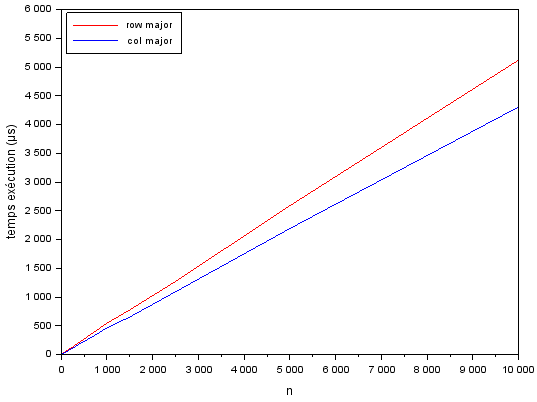
\includegraphics[scale=0.70]{time_dgbsv}
\caption*{\textit{Une partie du temps d'exécution sert à réinitialiser \texttt{RHS} car pour une meilleur mesure on répète le calcule mais dgbsv réécrit dans RHS, il faut donc le réinitialiser.}}
\end{figure}

\section{dgbmv}

\texttt{dgbmv} est une routine de \texttt{BLAS 2} qui calcule un \texttt{daxpy} entre matrice et vecteur de la forme \(y = \alpha Ax + \beta y\) où $\alpha$ et $\beta$ sont des scalaires.\footnote{netlib dgbmv : \href{http://www.netlib.org/lapack/explore-html/d7/d15/group__double__blas__level2_ga0dc187c15a47772440defe879d034888.html}{http://www.netlib.org/lapack/explore-html/[...].html}}
\begin{scriptsize}
\begin{minted}{c}
void cblas_dgbmv(CBLAS_LAYOUT layout,
                 CBLAS_TRANSPOSE TransA, const int M, const int N,
                 const int KL, const int KU, const double alpha,
                 const double *A, const int lda, const double *X,
                 const int incX, const double beta, double *Y, const int incY);
\end{minted}
\end{scriptsize}
La plupart des paramètres de la fonction s'utilise de la même manière que les fonctions utilisées précédemment. \texttt{M} est le nombre de lignes, \texttt{N} le nombre de colonnes. Il ne faut pas oublier que cette fonction n'effectue pas de factorisation \texttt{LU}, lorsqu'on construit la matrice \textit{band} $A$, il ne faut pas rajouter de diagonale supérieur supplémentaire (on a $\texttt{kv} = 0$). Deux \texttt{enum} sont réservé pour indiquer le layout, et le type de transposition de la matrice :
\begin{scriptsize}
\begin{minted}{c}
// cblas-netlib.h 
typedef enum {CblasRowMajor=101, CblasColMajor=102} CBLAS_LAYOUT;
typedef enum {CblasNoTrans=111, CblasTrans=112, CblasConjTrans=113} CBLAS_TRANSPOSE;
\end{minted}
\end{scriptsize}
On remarque que \texttt{LAPACKE} et \texttt{CBLAS} utilise la même norme pour indiquer le layout, la seul différence est que \texttt{CBLAS} utilise une enum alors que \texttt{LAPACKE} des \texttt{\#define} (voir \texttt{lapacke.h}). On a trois chois pour choisir le type de transposition : pas de transposition, transposition, ou bien transconjuguée (adjoint) en cas de matrice à coefficient complexe.
On remarque aussi que \texttt{dgbmv} est de type \texttt{void}, en regardant la doc netlib on voit que la gestion d'erreur se fait à l'intérieur de \texttt{dgbmv} via l'appel de la fonction \texttt{xerbla} qui print la variable locale \texttt{info} puis stoppe l'exécution du programme en cas d'erreur.

Dans notre cas, on fera appel à \texttt{dgbmv} pour calculer \(Ax\), où $A$ notre matrice \textit{band}, et $x$ notre vecteur solution analytique. Le résultat doit donc être \(Ax = f\) où $f$ est notre vecteur \texttt{RHS}. On doit donc mettre $\alpha = 1$ et $\beta = 0$. Notre matrice est carrée ($\texttt{la} \times \texttt{la}$), on a $\texttt{inX} = \texttt{incY} = 1$. Quant à la \texttt{leading dimension}, en \texttt{Col Major} : $\texttt{lda} = \texttt{kl} + \texttt{ku} + 1$. En \texttt{Row Major}, \texttt{lda} devrait être égale à la taille de la diagonale principale (\texttt{la}) mais ça ne fonctionne pas dû à un bug (on trouve une erreur relative $\approx 5.04$ pour $\texttt{la}=100$).
\begin{scriptsize}
\begin{minted}{c}
// appel de dgbmv en Col Major
cblas_dgbmv(CblasColMajor, CblasNoTrans, la, la, kl, ku, 1, AB, lab, EX_SOL, 1, 0, y, 1);
\end{minted}
\end{scriptsize}

On vérifie le résultat de la même manière que pour \texttt{dgbsv}, en mesurant l'erreur commise avec \(\frac{\lVert Ax - f \rVert_2}{\lVert f \rVert_2}\).

 \begin{table}[H]
\caption{dgbmv - Comparaison $Ax - f$}
\centering
\renewcommand*\arraystretch{1.1}
\begin{tabular}{|l|c|}
  \hline
  Nombre points (\texttt{la - 2}) & Erreur relative (Row Major) \\
  \hline
	27	&	\(8.74 \times 10^{-16}\) \\
	58	&	\(9.89 \times 10^{-16}\) \\
	102	&	\(6.40 \times 10^{-16}\) \\
	258	&	\(1.21 \times 10^{-15}\) \\
	999	&	\(5.08 \times 10^{-15}\) \\
  \hline
\end{tabular}
\end{table}
\begin{figure}[H]
\caption{Temps d'exécution \texttt{dgbmv}}
\centering
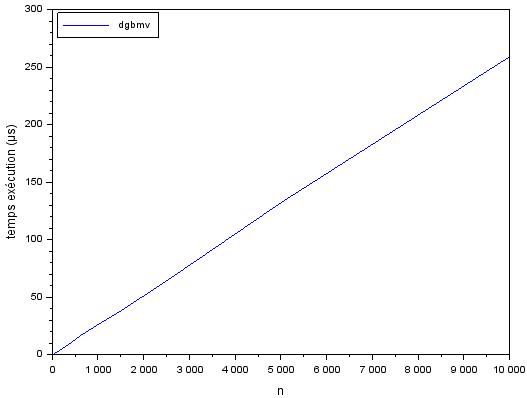
\includegraphics[scale=0.70]{time_dgbmv}
\end{figure}


\section{LU pour Poisson 1D}

D'après \texttt{scilab}, la factorisation $LU$ d'une matrice de Poisson 1D s'exprime simplement. $L$ et $U$ sont des matrices bidiagonale (respectivement \textit{lower} et \textit{upper}) où la diagonale principale de $L$ ne comporte que des 1, et la diagonale supérieur de $U$ ne comporte que des $-1$.
\[
	A = 
	\begin{pmatrix}
			2	& 	-1	&	0	& 0	\\
			-1	&	2	&\ddots	& 0	\\
			0	& \ddots&\ddots	&-1	\\
			0	& 	0	& -1 	& 2	\\
	\end{pmatrix}
\]
\[
	L = 
	\begin{pmatrix}
			1	& 	0	&	0	& 0	\\
			l_1	&	1	&	0	& 0	\\
			0	& \ddots&\ddots	& 0	\\
			0	& 	0	& l_{n-1} 	& 1	\\
	\end{pmatrix},
	U = 
	\begin{pmatrix}
			u_1	& 	-1	&	0	& 0	\\
			0	&	u_2	&\ddots	& 0	\\
			0	& 	0	&\ddots	& -1\\
			0	& 	0	& 0 	& u_n	\\
	\end{pmatrix}
\]
La représentation de $L$ et $U$ en format \textit{band} est :
\[
	L = 
	\begin{pmatrix}
		1	& 	1	&	1	&	\cdots	&	1		&	1	\\
		l_1	& 	l_2	&	l_3	&	\cdots	&	l_{n-1}	&	\ast	\\
	\end{pmatrix}
	\quad
	U = 
	\begin{pmatrix}
		\ast& 	-1	&	-1	&	\cdots	&	-1		&	-1	\\
		u_1	& 	u_2	&	u_3	&	\cdots	&	u_{n-1}	&	u_n	\\
	\end{pmatrix}
\]
Pour trouver les coefficients $\left\lbrace l_k \right\rbrace$ et $\left\lbrace u_k \right\rbrace$, on développe le produit $LU$

\[
	LU = 
	\begin{pmatrix}
			u_1		& 	-1		&	0				& 0		\\
			l_1 u_1	&	(u_2-l_1)	&\ddots				& 0		\\
			0		& 	\ddots	&\ddots				& -1	\\
			0		& 	0		& (l_{n-1} u_{n-1}) 	& (u_n-u_{n-1})	\\
	\end{pmatrix}
\]
En identifiant avec $A$, on obtient le système suivant :
\[
	\left \{
	\begin{array}{r c l}
		u_1 & = & 2 \\
		u_{n+1} - l_n & = & 2 \\
		l_n u_n & = & -1
	\end{array}
	\right .
	\Longrightarrow
	\left \{
	\begin{array}{r c l}
		l_1 = -\frac{1}{2} & , & u_1 = 2 \\
		u_{n+1} & = & 2 - \frac{1}{u_n} \\
		l_n & = & -\frac{1}{u_n}
	\end{array}
	\right .
\]
On implémente cet algorithme dans \texttt{lib\_poisson1D.c} en stockage \textit{band} dans la fonction \texttt{myluB\_colMajor\_poisson1D}. Il n'existe pas de fonction \texttt{dgbmm} dans \texttt{BLAS 3}, pour vérifier que notre résultat est bon, on effectue 2 produits matrice-vecteur \(L(Ux)\), où x est la solution exacte, puis on compare le résultat à \(f = \left[T_0\ 0\ 0\ \cdots 0\ T_1\right]\) (en norme-2).
On fait donc deux \texttt{dgbmv} avec $\beta = 0$, la \texttt{leading dimension} dans les deux cas est $2$. Entre les deux \texttt{dgbmv} on échange \texttt{EX\_SOL} et \texttt{y} pour obtenir le résultat final dans y.
\begin{scriptsize}
\begin{minted}{c}
  cblas_dgbmv(CblasColMajor, CblasNoTrans, la, la, 0, ku, 1, UB, 1 + ku, EX_SOL, 1, 0, y, 1); // Ux = y
  cblas_dswap(la, EX_SOL, 1, y, 1);
  cblas_dgbmv(CblasColMajor, CblasNoTrans, la, la, kl, 0, 1, LB, 1 + kl, EX_SOL, 1, 0, y, 1); // Lx =  y
\end{minted}
\end{scriptsize}
Puis on compare \texttt{y} et \texttt{RHS} ($f$) en norme-2 avec un \texttt{daxpy} et deux \texttt{ddot}.

On peut aussi implémenter cette algorithme en stockage dense puis vérifier le résultat avec une norme matricielle. Pour calculer la norme de $A$ on peut utiliser la fonction \texttt{dlange} de \texttt{LAPACK}, mais puisque $A$ est symétrique on peut tout aussi bien utiliser \texttt{dlansy} pour profiter de la symétrie de $A$.
\begin{scriptsize}
\begin{minted}{c}
double LAPACKE_dlansy( int matrix_layout, char norm, char uplo, lapack_int n, const double* a, lapack_int lda );
\end{minted}
\end{scriptsize}
Les matrices $A$, $L$ et $U$ sont écrites en \texttt{Row Major}. Comme norme on choisi par exemple la norme de Frobenius 'F'. Vu que $A$ contient tous les éléments des deux côtés de la diagonale, on peut choisir $\texttt{uplo} = 'U' ou 'L'$ indifféremment. \texttt{n} et \texttt{lda} sont tous deux égale à \texttt{lda} car $A$ est carré.

Pour calculer $LU-A$, on utilise \texttt{dgemm} de \texttt{BLAS 3}.
\begin{scriptsize}
\begin{minted}{c}
void cblas_dgemm(CBLAS_LAYOUT layout, CBLAS_TRANSPOSE TransA,
                 CBLAS_TRANSPOSE TransB, const int M, const int N,
                 const int K, const double alpha, const double *A,
                 const int lda, const double *B, const int ldb,
                 const double beta, double *C, const int ldc);
\end{minted}
\end{scriptsize}
$A$ est symétrique donc le \texttt{layout} importe peu, mais la factorisation $LU$ dans \texttt{mylu\_rowMajor\_poisson1D} est implémenté en \texttt{Row Major}. Aucune des matrice n'est transposé. \texttt{M}, \texttt{N}, \texttt{K}, et les \texttt{leading dimension} sont toutes égales à \texttt{la} car ce sont des matrices carrées.  
Pour calculer \( \lVert LU-A \rVert \) on utilise \texttt{dlange} de façon très similaire à \texttt{dlansy}.
\begin{scriptsize}
\begin{minted}{c}
temp = LAPACKE_dlansy(LAPACK_ROW_MAJOR, 'F', 'U', la, A, la);
cblas_dgemm(CblasRowMajor, CblasNoTrans, CblasNoTrans, la, la, la, 1, L, la, U, la,-1, A, la);
relres = LAPACKE_dlange(LAPACK_ROW_MAJOR, 'F', la, la, A, la);
\end{minted}
\end{scriptsize}\begin{table}[H]
\caption{Factorisation LU - Comparaison $LU - A$}
\centering
\renewcommand*\arraystretch{1.1}
\begin{tabular}{|l|c|c|}
  \hline
  \texttt{la} & Err. rel. (Band, Col Major) & Err. rel. (Dense, Row Major) \\
  \hline
	25	&	\(9.53 \times 10^{-16}\)	&	\(0.00\) \\
	56	&	\(1.01 \times 10^{-15}\)	&	\(8.59 \times 10^{-18}\) \\
	100	&	\(7.66 \times 10^{-16}\)	&	\(6.42 \times 10^{-18}\) \\
	256	&	\(1.38 \times 10^{-15}\)	&	\(4.00 \times 10^{-18}\) \\
	999	&	\(3.20 \times 10^{-15}\)	&	\(2.48 \times 10^{-18}\) \\
  \hline
\end{tabular}
\end{table}
\begin{figure}[H]
\caption{Temps d'exécution \texttt{LU} band et dense}
\centering
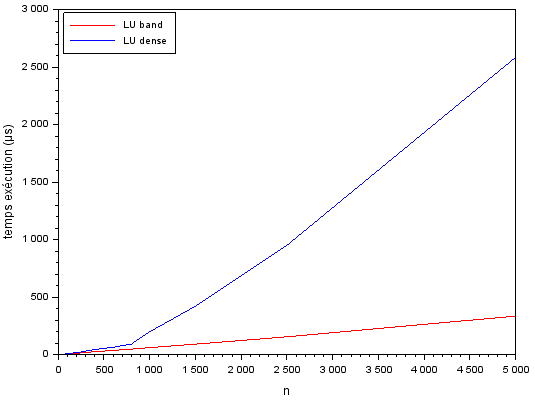
\includegraphics[scale=0.70]{time_lu_band_dense}
\caption*{\textit{Pour de grand n, le temps de vérification de $LU$ \textit{dense} devient très long dû aux \texttt{dlan**} et \texttt{dgemm}.}}
\end{figure}
Les fonctions initialisent $2n$ éléments pour chaque matrice $L$ et $U$, la complexité théorique des algorithmes est donc en \(\mathcal{O}(4n)\).
On remarque que le temps de construction de $LU$ dense explose alors que les deux algorithmes initialise le même nombre d'élément. On peut expliquer la différence par la proximité en mémoire des éléments non nuls du format \textit{band} par rapport au format \textit{dense} : une plus grande partie des éléments à initialiser du tableau \textit{band} rentre en mémoire cache.

\section{Jacobi et Richardson \texttt{Scilab}}
L'itération de Richardson s'écrit : 
\[
	\begin{array}{r c l r}
		x^{k+1} & = & x^k + \alpha(b-Ax^k) & \quad avec\ \alpha > 0
	\end{array}
\]
On peut la réécrire sous la forme :
\[
	\begin{array}{r c l}
		x^{k+1} & = & (I-\alpha A)x^k + \alpha b \\
		 		& = & G_\alpha x^k + \alpha b
	\end{array}
\]
Pour que le processus converge, il faut que $\rho (G_\alpha) < 1$, où :
\[
	\begin{array}{r c l}
		\rho (G_\alpha) & = & max\left\lbrace \left| \lambda_G \right|,\ \lambda_G\in\lambda (G_\alpha)\right\rbrace
	\end{array}
\]
On peut encadrer les $\lambda_G$ par les valeurs propres de $A$.
\[
	\begin{array}{r c l r}
		Ax & = & \lambda x & \quad \lambda_{min} \leq \lambda \leq \lambda_{max}\\
		(I-\alpha A)x & = & (1-\alpha \lambda) x &\\
		G_\alpha x & = & (1-\alpha \lambda) x &\\
	\end{array}
\]
On cherche donc un $\alpha$ tel que :
\[
	\left \{
	\begin{array}{r c l}
		\left| 1 - \alpha \lambda_{min} \right| < 1 \\
		\left| 1 - \alpha \lambda_{max} \right| < 1 \\
	\end{array}
	\right .
\]
\begin{itemize}
\item Si 
\[
	\begin{array}{r c l}
		1 - \alpha \lambda \leq 0 & , \quad \lambda > 0 \\
		\alpha \geq \frac{1}{\lambda} & \\
	\end{array}
\]
Alors, 
\[
		\alpha \lambda - 1 < 1 \quad
		\Rightarrow \quad \alpha < \frac{2}{\lambda}
\]
Et on a donc :
\[
		\frac{1}{\lambda} \leq \alpha < \frac{2}{\lambda}
\]
\item Si 
\[
	\begin{array}{r c l}
		1 - \alpha \lambda \leq 0 & , \quad \lambda < 0 \\
		\alpha \leq \frac{1}{\lambda} & \\
	\end{array}
\]
Alors, $\alpha$ doit être négatif, c'est impossible.
\item Si 
\[
	\begin{array}{r c l}
		1 - \alpha \lambda & \geq & 0 \\
		\alpha & \leq & \frac{1}{\lambda} \\
	\end{array}
\]
Alors, 
\[
		1 - \alpha \lambda < 1 \quad
		\Rightarrow \quad -\alpha \lambda < 0 \quad
		\Rightarrow \quad \lambda > 0
\]
Et on a donc :
\[
		0 < \alpha \leq \frac{1}{\lambda}
\]
\end{itemize}
On a donc l'encadrement suivant :
\[
	0 < \alpha < \frac{2}{\lambda}
\]
Le $\alpha$ optimal minimise tous les $\left| 1 - \alpha \lambda \right|$. On trace les courbe associées $\lambda_{min}$ et $\lambda_{max}$ pour le trouver :
\begin{figure}[H]
\caption{Courbes $\left| 1 - \alpha \lambda \right|$}
\centering
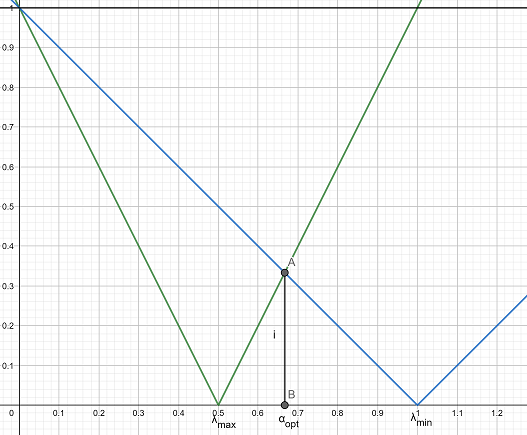
\includegraphics[scale=0.70]{alpha_opt}
\end{figure}
$\alpha_{opt}$ est à l'intersection des courbes après qu'une ai été reflété. On a donc :
\[
	1 - \alpha_{opt} \lambda_{min} = \alpha_{opt} \lambda_{max} - 1
\]
\[
	\alpha_{opt} = \frac{2}{\lambda_{min} + \lambda_{max}}
\]
Pour trouver les valeurs propre de on utilise la fonction \texttt{spec} de \texttt{scilab}. On trouve que quelque soit la taille de $A$, $\lambda_{min} + \lambda_{max} = 4$, on a donc $\alpha_{opt} = \frac{1}{2}$.
On implémente l'algorithme en \texttt{scilab} puis on trace les courbes d'erreurs (par rapport à la solution analytique) en fonction de $\alpha$ :
\begin{figure}[H]
\caption{Erreur Richardson pour n = 100}
\centering
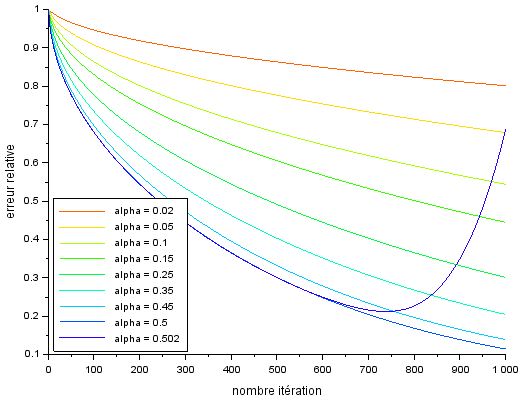
\includegraphics[scale=0.70]{conv_richardson_n100}
\end{figure}
On retrouve que pour un $\alpha$ très légèrement supérieur à $\alpha_{opt}$, le processus de Richardson diverge.


\end{document}
